% Chapter 13

\chapter{Conclusions and Outlook} % Chapter title
\label{ch:conc} 

After a series of moderate excesses observed by the ATLAS experiment in events with a $Z$ boson, jets, and \met, this analysis performed on 14.7 fb$^{-1}$ of 13 \tev~data sees excellent agreement between observations and the background expectation. The resulting exclusion pushes the gluino mass lower limit beyond 1 \tev, putting further constraints on possible \ac{SUSY} models. Along with the many other searches for \ac{SUSY}, this exclusion limits the phase space available for natural \ac{SUSY} models. However, \ac{SUSY} is adaptable; new theories stretching those bounds are continually proposed as tighter experimental constraints are set, and there are always small gaps in the exclusions where sparticles could hide. 

ATLAS's dataset for 2016 includes 36 fb$^{-1}$, more than twice the luminosity included in this search. Because no excess was seen in this analysis, the next search in this channel will be able to re-optimize its signal regions for this larger dataset. In fact, because the signal region has been frozen since the 8 \tev~search, this analysis's signal region hasn't ever been re-optimized for the increased energy of the \ac{LHC}'s collisions. A new signal region that increases \met and \HT requirements will allow for better sensitivity to \ac{SUSY} processes. 

In addition, the current signal region, in which 60 events were observed with 14.7 fb$^{-1}$, will be populated enough to be subdivided based on event features. The current search is agnostic to the number of $b$-jets in the event, for example, but there are now enough events to separate this signal region into complementary $b$-tagged and $b$-vetoed regions, allowing analyzers to independently target models which produce $b$-jets and those that don't, and in the latter case, to dramatically reduce the \ttbar background. Signal regions can also be binned in other model-dependent features, like number of jets, and the \met and \HT requirements can be increased independently, targeting different event topologies. 

The \ac{LHC} will continue to run through 2018 with a possible increase to $\sqrt{s} = 14\tev$, and will shut down for upgrades until 2021. Three more years of data-taking at $14\tev$ will follow, with approximately twice the current luminosity, referred to as Run 3. After that, the \ac{LHC} will shut down again to prepare for the \ac{HL-LHC}, which will begin data-taking in 2026 at a luminosity approximately five times the current rate. This run will result in roughly 3000 fb$^{-1}$, which will allow for dramatically better sensitivity in \ac{SUSY} searches. An example can be seen in \autoref{fig:conc_hllhc}, which shows the potential exclusions on a simple gluino pair-production model with decays via squarks to a \ac{LSP}, for the approximate luminosities of Run 3 and the \ac{HL-LHC}. 

\begin{figure}[!htb]
\centering
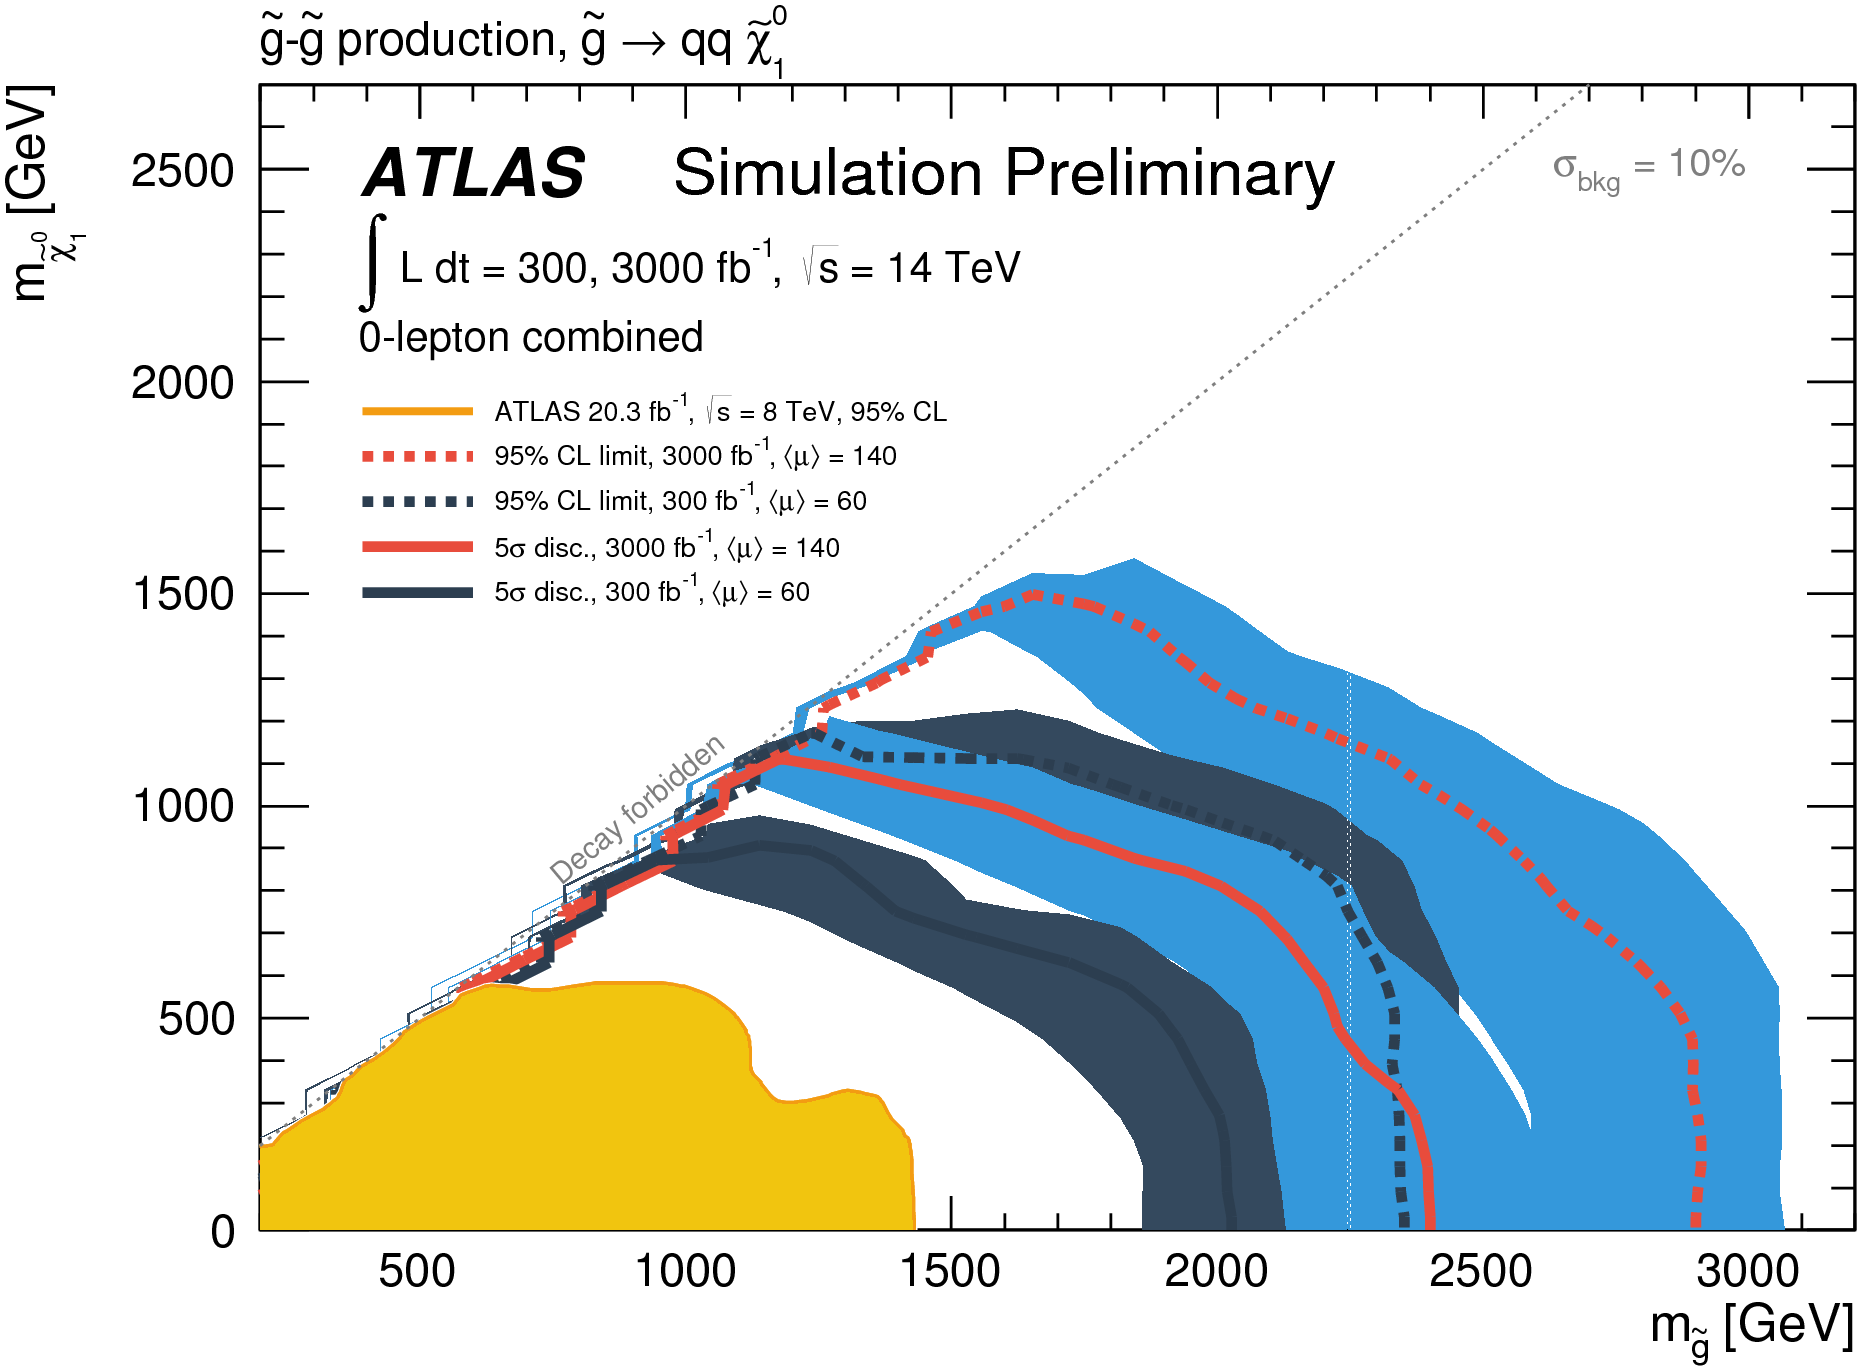
\includegraphics[width=.9\textwidth]{figures/interpretation/fig_09a.png}
\caption{ Expected 95\% \ac{CL} exclusion contours (dashed) and 5$\sigma$ discovery contours (solid) for $L_{int} = 300^{-1}$ (black) and $3000^{-1}$ (red) for gluino pair-production, with 1$\sigma$ bands representing the uncertainty on the production cross-section. Superimposed is the observed 8 \tev~exclusion for similar models. \cite{ATL-PHYS-PUB-2016-022}}
\label{fig:conc_hllhc}
\end{figure}

Searches like this one will surely be repeated with higher and higher luminosities, the analyses increasing both in sensitivity and in complexity. Whether or not they uncover any hints of physics beyond the Standard Model remains to be seen. 



%----------------------------------------------------------------------------------------
